\documentclass[a4paper,10pt]{article}
\usepackage[utf8]{inputenc}
\usepackage{amsmath, amssymb}
\usepackage{graphicx}
\usepackage{caption}
\usepackage{subcaption}
\usepackage{pgffor}
\usepackage{arrayjob}

% Define arranjos
\newarray\hpbw
\newarray\ganho

% preenche arranjos
\readarray{hpbw}{240.00&
		 180.00&
		 149.86&
		 131.06&
		 117.06&
		 108.05&
		 100.31&
		 94.03&
		 88.79&
		 84.34} 
		 
\readarray{ganho}{-1.99&
		  1.04&
		  2.64&
		  3.80&
		  4.72&
		  5.48&
		  6.12&
		  6.68&
		  7.18&
		  7.63}

\title{\vspace{-3cm}Universidade Federal do Ceará\\Sistemas de Comunicações Móveis\\Primeiro Trabalho Computacional}
\author{Lucas Nogueira Ribeiro}
\date{}

\begin{document}
\maketitle

Considere uma antena com padrão de irradiação de potência dado por 
\begin{equation}
 P(\theta) = \cos^n(\theta / 2),\quad \theta \in [-\pi, \pi], \, n \geq 0.
\end{equation}
Sabe-se que o \emph{half-power beamwidth} (HPBW) é definido como o intervalo ângular formado pelos pontos de meia potência, i.e. $P(\theta) = 0.5$. O ângulo de meia potência pode ser expresso como
\begin{equation}
 \theta = 2\cos^{-1}\left( \sqrt[n]{0.5} \right)
\end{equation}
A fórmula para o cálculo do HPBW é dada por
\begin{equation}
 \text{HPBW} = 2\theta = 4\cos^{-1}\left( \sqrt[n]{0.5} \right)
\end{equation}

O cálculo do ganho desta antena pode ser feito através da fórmula de Kraus, que aproxima a diretividade $D$ da antena através do seu HPBW. Esta fórmula é dada por \cite{balanis}:
\begin{equation}
 D = \frac{41253}{\textrm{HPBW}^2\, \text{[graus]}}
\end{equation}
A relação entre o ganho $G$ e a diretividade $G$ de uma antena é dada pela equação $G=\eta D$, em que $\eta \in \mathbb{R}$ é a eficiência da antena. Considerou-se $\eta=1$ neste trabalho. Portanto, $G=D$. O ganho em decibéis (dB) desta antena em relação à antena isotrópica é dado por
\begin{equation}
 G\,[\text{dBi}] = 10\log_{10}D = 10\log_{10}\left\{ \frac{41253}{\left[ \cos^{-1}\left( \sqrt[n]{0.5} \right) \right]^2} \right\}
\end{equation}	

O padrão de irradiação de potência das antenas ($n=1,\ldots,10$) foi mostrado juntamente com o seu ganho e HPBW nas Figuras \ref{fig:1} a \ref{fig:10}. Observou-se que o ganho e o HPBW da antena aumentaram com o valor de $n$. Estes valores foram plotados em função do parâmetro $n$ nas Figuras \ref{fig:ganho} e \ref{fig:hpbw}. Observou-se um aumento importante na diretividade de $n=1$ até $n=10$. A partir de então, o aumento na diretividade não foi tão importante. Como o parâmetro $n$ normalmente está relacionado a fatores físicos da antena que podem aumentar o seu custo, observa-se, portanto, um compromisso entre o ganho da antena e o seu parâmetro $n$.

\cleardoublepage
\foreach \n in {1,...,10}{
  \begin{figure}[t!]
      \centering
      \begin{subfigure}[t]{0.48\textwidth}
	  \centering
	  \includegraphics[width=1.1\textwidth]{./figuras/radlin_n\n.eps}
	  \caption{Plot linear}
	  \label{fig:linear\n}
      \end{subfigure} %
      ~
      \begin{subfigure}[t]{0.48\textwidth}
	  \centering
	  \includegraphics[width=1.1\textwidth]{./figuras/radpol_n\n.eps}
	  \caption{Plot polar}
	  \label{fig:polar\n}
      \end{subfigure}
      \caption{Plots de $P(\theta)$ para $n=\n$. $\text{Ganho} = \protect\ganho(\n)\,\text{dBi}$, $\text{HPBW} = \protect\hpbw(\n)$.}
      \label{fig:\n}
  \end{figure}
}

\begin{figure}
 \centering
 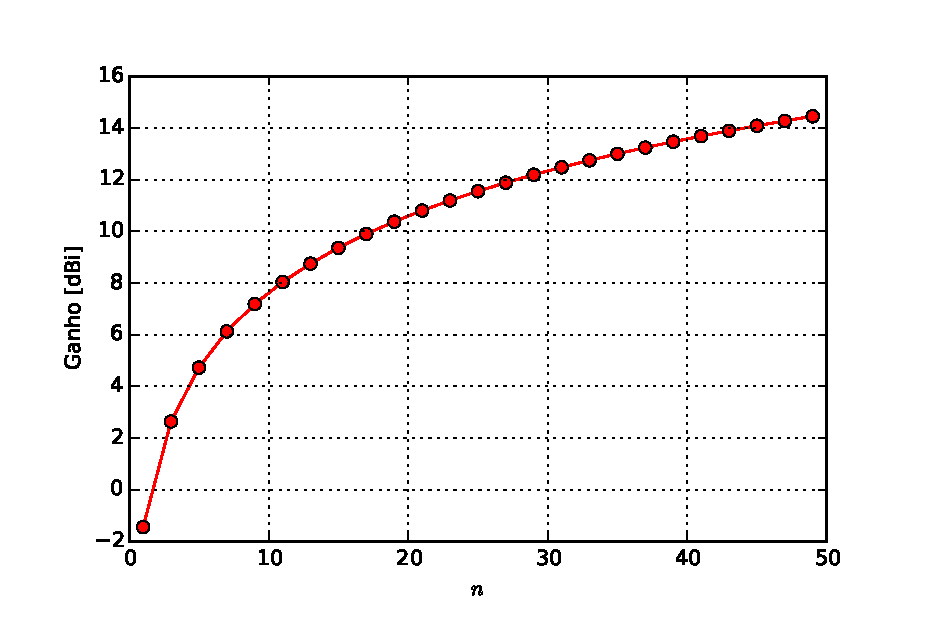
\includegraphics[width=0.8\textwidth]{./figuras/n_vs_ganho.eps}
 \caption{Ganho da antena em função do parâmetro $n$.}
 \label{fig:ganho}
\end{figure}

\begin{figure}
 \centering
 \includegraphics[width=0.8\textwidth]{./figuras/n_vs_hpbw.eps}
 \caption{HPBW em função do parâmetro $n$.}
 \label{fig:hpbw}
\end{figure}

\cleardoublepage
\section*{Código fonte}
O código fonte Python escrito para gerar as figuras deste trabalho é mostrado abaixo.

\begin{verbatim}
import numpy as np
import matplotlib.pyplot as plt

p = lambda t, n : np.cos(t/2.0)**n # padrão de potência 
g_kraus = lambda n: 10*np.log10(41253./(hpbw(n)**2.)) # Fórmula de Kraus
hpbw = lambda n: 4*np.math.degrees(np.math.acos((0.5)**(1./n)))

def plotDiagramaRadiacao(n):
    print 'Ganho - Kraus[{}]: {} [dBi]'.format(n, g_kraus(n))
    print 'HPBW[{}]: {} [graus]'.format(n, hpbw(n))
    print
    
    ang = np.radians(0.5*hpbw(n))
    theta = np.linspace(-np.pi, np.pi, 1000)
    theta_ticks = np.linspace(-np.pi, np.pi, 7)

    # plot linear
    plt.figure()
    plt.plot(theta, p(theta, n),linewidth=2)
    plt.xticks(theta_ticks, np.degrees(theta_ticks))
    plt.plot(ang*np.array([1, 1]), [0, 1], '--k')
    plt.plot(-ang*np.array([1, 1]), [0, 1], '--k')
    plt.xlabel('$\\theta$ [graus]')
    plt.ylabel('$P(\\theta)$')
    plt.title('$n={}$'.format(n))
    plt.grid()

    # plot polar
    plt.figure()
    plt.polar(theta, p(theta, n),linewidth=2)
    plt.plot(ang*np.array([1, 1]), [0, 1], '--k')
    plt.plot(-ang*np.array([1, 1]), [0, 1], '--k')
    plt.title('$n={}$'.format(n), loc='left') # parâmetro y afasta o title
    
    for n in np.arange(1,11):
    plotDiagramaRadiacao(n)
    
ganho_kraus = []
ganho_tp = []
meiapot = []

nrange = np.arange(1,51,2)

for n in nrange:
    ganho_kraus.append(g_kraus(n))
    meiapot.append(hpbw(n))
    
plt.figure()
plt.plot(nrange, ganho_kraus, '-ro')
plt.xlabel('$n$')
plt.ylabel('Ganho [dBi]')
plt.grid()


plt.figure()
plt.plot(nrange, meiapot, '-bo')
plt.xlabel('$n$')
plt.ylabel('HPBW [graus]')
plt.grid()
\end{verbatim}
\begin{thebibliography}{9}

\bibitem{balanis}
  Balanis, Constantine A. 
  \emph{Antenna theory: analysis and design.},
  Vol. 1.
  John Wiley \& Sons, 2005.
\end{thebibliography}

\end{document}
